%% Template article for preprint document class `elsart'
%% SP 2001/01/05
%

\documentclass{elsart}

% Use the option doublespacing or reviewcopy to obtain double line spacing
% \documentclass[doublespacing]{elsart}

% if you use PostScript figures in your article
% use the graphics package for simple commands
%\usepackage{graphics}
% or use the graphicx package for more complicated commands
% \usepackage{graphicx}
% or use the epsfig package if you prefer to use the old commands
\usepackage{epsfig}
\usepackage{subfigure}
% The amssymb package provides various useful mathematical symbols
\usepackage{amssymb}
\usepackage{multirow}
\usepackage{rotating}
%\usepackage{booktabs}
% The lineno packages adds line numbers. Start line numbering with
% \begin{linenumbers}, end it with \end{linenumbers}. Or switch it on
% for the whole article with \linenumbers.
% \usepackage{lineno}

% \linenumbers
\begin{document}

\begin{frontmatter}

% Title, authors and addresses

% use the thanksref command within \title, \author or \address for footnotes;
% use the corauthref command within \author for corresponding author footnotes;
% use the ead command for the email address,
% and the form \ead[url] for the home page:
% \title{Title\thanksref{label1}}
% \thanks[label1]{}
% \author{Name\corauthref{cor1}\thanksref{label2}}
% \ead{email address}
% \ead[url]{home page}
% \thanks[label2]{}
% \corauth[cor1]{}
% \address{Address\thanksref{label3}}
% \thanks[label3]{}

\title{A Study of Feature Selection and Sampling Techniques for Predicting Defective Software Modules}

% use optional labels to link authors explicitly to addresses:
% \author[label1,label2]{}
% \address[label1]{}
% \address[label2]{}

% \author[a]{Daniel Rodr\'iguez}
% \author[b]{Israel Herraiz}
% \author[c]{Roberto Ruiz}
% \author[d]{J.C. Riquelme}
%
% \address[a]{Dept of Computer Science\\
%     The University of Alcal\'a\\
%     Ctra Barcelona Km 37,1\\
%     28805 Alcal\'a de Henares, Madrid, Spain
%     }
% \address[b]{Dept of Computer Science\\
%     University Pablo de Olavide\\
%     Ctra Utrera Km 1\\
%     41013 Sevilla, Spain}
% \address[c]{Dept of Computer Science\\
%     The University of Seville\\
%     Ctra Utrera Km 1\\
%     41013 Sevilla, Spain}






%%%%%%%%%%%%%%%%%%%%%%%%%%%%%%%%%%%%%%%%%%%%%%%%%%%%%%%%%%%%%%%%%%%%%%
%%%%%%%%%%%%%%%%%%%%%%%%%%%%%%%%%%%%%%%%%%%%%%%%%%%%%%%%%%% Abstract %
%%%%%%%%%%%%%%%%%%%%%%%%%%%%%%%%%%%%%%%%%%%%%%%%%%%%%%%%%%%%%%%%%%%%%%


\begin{abstract}



This paper presents a study of applying Feature Selection (FS) and sampling techniques for predicting defective modules using data from a publicly available repository. In general, FS maintains or even improves the accuracy of predictions. However, many software engineering datasets tend to be highly unbalanced, i.e. a large number of instances in a class (majority class) outweighs the number of instances in the minority class. In this case, classification results can be misleading, as good predictions can be obtained selecting the majority class. However, the accuracy for the minority class, which is generally the interesting one to predict (defective modules in this case), tends to be very low. Results show that sampling and FS techniques can help to better predict defective modules. Also, in relation to FS, the subset of attributes can help to characterise and the subset of attributes may also be affected by the sampling techniques. Finally, in relation to measure the goodness of the classifier, the percentage of corrected classified instances is not a good indicator and other measures such as area under the curve and the rate of true negatives could be considered when evaluating the accuracy of the classifier.
\end{abstract}

\begin{keyword}
% keywords here, in the form: keyword \sep keyword
Software defects \sep Feature Selection \sep Sampling techniques
Unbalanced databases
 \sep Na\"ive Bayes classifier
% PACS codes here, in the form: \PACS code \sep code
\PACS
\end{keyword}


\end{frontmatter}


%%%%%%%%%%%%%%%%%%%%%%%%%%%%%%%%%%%%%%%%%%%%%%%%%%%%%%%%%%%%%%%%%%%%%
%%%%%%%%%%%%%%%%%%%%%%%%%%%%%%%%%%%%%%%%%%%%%%%%%%%%%% Introduction %
%%%%%%%%%%%%%%%%%%%%%%%%%%%%%%%%%%%%%%%%%%%%%%%%%%%%%%%%%%%%%%%%%%%%%

\section{Introduction}
\label{sec:intro}


At present, automated data collection tools allow us to collect large amounts of information, but not without associated problems.
In this paper, we analyse the application Feature Selection (FS, also known as attribute selection or Feature Subset Selection -FSS-) and sampling techniques with highly unbalanced datasets from the PROMISE repository\footnote{\texttt{http://promisedata.org/}}\cite{PROMISERep} for predicting defective modules.

On the one hand, a large number of attributes in a dataset makes more difficult the application of techniques such as regression or classification. The need of applying FS includes the following items:
\begin{itemize}
  \item A reduced volume of data allow us to apply different data mining or searching techniques.

  \item Irrelevant and redundant attributes can generate less accurate and more complex models. Furthermore, data mining algorithms can be executed faster.

  \item It is possible to avoid the collection of data for those irrelevant and redundant attributes in the future.
\end{itemize}

In a previous work~\cite{Rodriguez2007AttSelection}, we analysed the application of FS for classifying defective modules. The results, however, can be affected by the problem of unbalanced datasets. With unbalanced datasets, i.e. instances of one class heavily outnumber the instances in the other class when trying to characterize databases in Software Engineering can arise two main of problems~\cite{Kitchenham2007UnbalancedDS}: (i) the impact of some factors can be concealed, and (ii) spurious impacts may be observed. When learning with data mining algorithms, the generated models may also be affected as most learners assume balanced datasets and it is possible to obtain apparently good overall accuracy predictions that are misleading. For example, if we have an unbalanced dataset with two classes, the majority class with 95\% of its instances and a minority class with the remaining 5\%, we can obtain an accuracy of 95\% just by always selecting the majority class. The classifier, however, fails for the minority class which is the one we are generally interested in finding. In the case of this work, the minority class is the one that indicates defective modules. There are two approaches when dealing with unbalanced datasets, one is to improve the classification algorithms to make them more robust to unbalanced datasets or the other approach is to use sampling techniques. In this work, sampling techniques were used to generate new datasets that improve distribution of instances across the classes. This may not always to increase the overall accuracy but it tends to increase the accuracy for the minority class.

The rest of the paper is organized as follows. Section~\ref{sec:background} explains briefly the background behind FS, balancing techniques, the classifier selected and common evaluation techniques and measures used in this work. Section~\ref{sec:experimentalResults} describes the experimental results of applying FS and sampling techniques to several datasets from the PROMISE repository, followed by some related works in Section~\ref{sec:relatedWork}. Finally, conclusions and future work are commented in Section~\ref{sec:conclusions}.


%As an example, the CM1 dataset used in this work and described later
%is composed of 498 instances and 22 attributes. The majority class
%(no-defects) contains 449 instances and the minority class (defects)
%only contains 49 instances. A standard classification using the C4.5
%algorithm provided by the Weka tool produces the following results:
%
%\begin{small}
%\begin{verbatim}
%Correctly Classified    438   87.95%
%Incorrectly Classified   60   12.04 %
%...
%=== Confusion Matrix ===
%   a   b   <-- classified as
% 435  14 |   a = false
%  46   3 |   b = true
%\end{verbatim}
%\end{small}
%
%
%In the confusion matrix, it can observed that it fails 46 times out of 49 times when classifying the defective module. To deal with this problem, it is possible to apply balancing techniques. For example, we can resample instances to obtain a new dataset by replicating the number of instances following the original dataset distribution for each class and uniform distribution between the classes (defective or non-defective). In this case, the same standard classification technique with new dataset, which is composed of 996 instances, obtains the following results:
%
%%However, after applying the balancing technique, Resample, we
%%obtain a dataset with 996 instances with uniform distribution
%%between the classes (the number of instances is doubled so that
%%there is approximately the same number instances of the majority and
%%minority class. This is achieved by replicating the number of instances following the original dataset distribution for each class and normalizing the distribution of the classes). The summary of the results obtained is as follows:
%
%\begin{small}
%\begin{verbatim}
%Correctly Classified    956   95.98%
%Incorrectly Classified  40     4.01%
%...
%=== Confusion Matrix ===
%   a   b   <-- classified as
% 434  40 |   a = false
%   0 522 |   b = true
%
%\end{verbatim}
%\end{small}
%
%
%The results show that by balancing the majority and
%minority class not only the overall accuracy has improved. but also the accuracy of the minority class has greatly improved (in fact, there is a 100\% accuracy for the minority class in this case).
%
%In addition to balancing techniques, it is possible to apply FS to the previous resampled dataset. The results show that the overall accuracy remains similar (94.8\% compared to 95.9\%), however
%this level of accuracy is obtained only with 5 attributes instead of the 22 original attributes.
%
%\begin{small}
%\begin{verbatim}
%Correctly Classified   945    94.87%
%Incorrectly Classified  51     5.12%
%...
%=== Confusion Matrix ===
%   a   b   <-- classified as
% 423  51 |   a = false
%   0 522 |   b = true
%\end{verbatim}
%\end{small}



%%%%%%%%%%%%%%%%%%%%%%%%%%%%%%%%%%%%%%%%%%%%%%%%%%%%%%%%%%%%%%%%%%%%%%%%%
%%%%%%%%%%%%%%%%%%%%%%%%%%%%%%%%%%%%%%%%%%%%%%%%%%%%%%%%%%% Background %%%
%%%%%%%%%%%%%%%%%%%%%%%%%%%%%%%%%%%%%%%%%%%%%%%%%%%%%%%%%%%%%%%%%%%%%%%%%%
\section{Background}
\label{sec:background}

%%%%%%%%%%%%%%%%%%%%%%%%%%%%%%%%%%%%%%%%%%%%%%%%%%%%%%%%%%%%%%%%%%%%%%%%%%
\subsection{Feature Selection (FS)}
\label{subSec:featureSelection}
%
The problem of Feature Selection (FS) has received a thorough treatment in pattern recognition and machine learning. Most of the
FS algorithms tackle the task as a search problem, where each state in the search specifies a distinct subset of the possible
attributes~\cite{BL97}. The search procedure is combined with a criterion to evaluate the merit of each candidate subset of
attributes. There are a multiple possible combinations between each procedure search and each attribute measure\cite{LY05}. There are various ways in which FS algorithms can be classified depending on the type (filter or wrapper techniques) or on the way that features are evaluated (individual or subset evaluation)~\cite{BL97,Lan94,LM98,LY05,LY04}:%DL97,

\begin{itemize}
  \item The \emph{filter model} relies on general characteristics of the data to evaluate and select feature subsets without involving any data mining algorithm.

  \item The \emph{wrapper model} requires one predetermined mining algorithm and uses its performance as the evaluation criterion. It searches for features better suited to the mining algorithm aiming to improve mining performance, but it also tends to be more computationally expensive than the filter model~\cite{KJ97,Lan94}.
\end{itemize}


%As mentioned earlier, there exist two major approaches in feature
%selection from the method's output point of view: feature ranking
%and feature subset selection (FSS), which depend on the way that
%features are evaluated.


Feature Ranking (FR)~\cite{BL97,GE03}, also called feature weighting, assesses individual features and assigns them weights
according to their degrees of relevance %, while the
%second one evaluates the goodness of each found feature
%subset~\cite{LM98}. (Unusually, some search strategies in
%combination with subset evaluation can provide a ranked list).
In the FR algorithms category, one can expect a ranked list of features which are ordered according to evaluation measures. A subset of features is often selected from the top of a ranking list. A feature is good and thus will be selected if its weight of
relevance is greater than a user-specified threshold value.

%or we can simply select the first $k$ features from the ranked list. This
%approach is efficient for high-dimensional data due to its linear
%time complexity in terms of dimensionality.

Candidate feature subsets are generated based on a certain search strategy and evaluation measure which captures the goodness of each subset. Each candidate subset is evaluated by a certain evaluation measure and compared with the previous best one with respect to this measure. If a new subset turns out to be better, it replaces the previous best subset. The process of subset generation and evaluation is repeated until a  stopping criterion is satisfied. Different algorithms address theses issues differently. In~\cite{LY04}, a large number of selection methods are categorized. We found different search strategies, namely exhaustive, heuristic and random search, combined with several type of measures to form different algorithms.

%The time
%complexity is exponential in terms of data dimensionality for
%exhaustive search and quadratic for heuristic search. The complexity
%can be linear to the number of iterations in a random
%search~\cite{LS96a}, but experiments show that in order to find best
%feature subset, the number of iterations required is mostly at least
%quadratic to the number of features~\cite{DLM00}.


FS algorithms search through candidate feature subsets guided by a certain evaluation measure~\cite{LM98} which captures the goodness of each subset. Some existing evaluation measures that have been shown effective in removing both irrelevant and redundant features include the consistency measure~\cite{DLM00}, the correlation measure \cite{Hall99CFSThesis} and the estimated accuracy of a learning algorithm~\cite{KJ97}:

\begin{itemize}
\item \emph{Consistency measure} (CNS) attempts to find a minimum number of features that separate classes as consistently as the full set of features can. An inconsistency is defined as the instances having the same feature values but different class labels.

\item \emph{Correlation measure} (CFS) evaluates the goodness of feature subsets based on the hypothesis that good feature subsets contain features highly correlated to the class, yet uncorrelated to each other.

\item \emph{Wrapper-based} (WP) attribute selection uses the target learning algorithm to estimate the worthiness of attribute subsets. The feature subset selection algorithm conducts a search for a good subset using the induction algorithm itself as part of the evaluation function.

\end{itemize}


Langley~\cite{Lan94} notes that FS algorithms that search through the space of feature subsets must address four main issues: (i) the starting point of the search, (ii) the organization of the search, (iii) the evaluation of features subsets and (iv) the criterion used to terminate the search. Different algorithms address theses issues differently.

It is impractical to look at all possible feature subsets, even for small datasets. Feature selection algorithms usually proceed
greedily. They can be classified into those that add features to an initially empty set (\emph{forward selection}) and those that remove features from an initially complete set (\emph{backward elimination}). They can also be \emph{hybrid} if features can be
both added and removed as the algorithm progresses. Forward selection is much faster than backward elimination and therefore
scales better to large data sets. Also, a wide range of search strategies can be used: best--first, branch--and--bound, simulated
annealing, genetic algorithms (see Kohavi and John~\cite{KJ97} for a review).

In this paper, two widely used evaluation methods provided by the Weka toolkit~\cite{WF05}, correlation and consistency. Correlation-based Feature Selection (CFS)~\cite{Hall99CFSThesis}, which is based on test theory, searches subsets of attributes highly correlated with the class but having a low correlation between them. The consistency method (CNS)~\cite{DLM00}, a probabilistic approach, searches for the smallest subset of attributes such that the level of consistency in the class values is equal to the full set of attributes. In both cases, the selection of attributes for the correlation and consistency methods was performed following a sequential search with greedy forward selection in the space of attributes.

%In \cite{DLM00}, different search strategies, namely exhaustive,
%heuristic and random search, are combined with consistency measure
%to form different algorithms. The time complexity is exponential in
%terms of data dimensionality for exhaustive search and quadratic for
%heuristic search. The complexity can be linear to the number of
%iterations in a random search~\cite{LS96a}, but experiments show
%that in order to find best feature subset, the number of iterations
%required is mostly at least quadratic to the number of
%features~\cite{DLM00}. In \cite{Hal99}, correlation measure is
%applied in an algorithm called CFS that exploit heuristic search
%(best first) to search for candidate feature subsets.
%
%One of the most frequently used search techniques is hill-climbing
%(greedy). It starts with an empty set and evaluates each attribute
%individually to find the best single attribute. It then tries each
%of the remaining attributes in conjunction with the best to find the
%most suited pair of attributes. In the next iteration, each of the
%remaining attributes are tried in conjunction with the best pair to
%find the most suited group of three attributes. This process
%continues until no single attribute addition improves the evaluation
%of the subset; i.e., subset evaluator is run \emph{M} times to
%choose the best single attribute, \emph{M-1} times to find the best
%pair of attributes, \emph{M-2} times the best group of three, and so
%on. For example, if we have chosen five attributes through this
%method, the subset evaluator has been run
%\emph{M+(M-1)+(M-2)+(M-3)+(M-4)} times.
%
%Recently, Yu and Liu~\cite{YL04b} proposed a new framework of FS,
%fast correlation--based filter algorithm (FCBF) which uses
%correlation measure to obtain relevant genes and to remove
%redundancy. There are other methods based on relevance and
%redundancy concepts. It is based on the concept of Markov blanket,
%where $M$ is formed by only one attribute, and gradually eliminates
%redundant attributes with respect to $M$ from the first to the final
%attribute of an ordered list.

%This algorithm is among the most cited work at present following the above--mentioned framework (FR+FSS).

%%% la descri�n m�s completa en espa�ol
%El algoritmo FCBF (\emph{Fast Correlation-Based Filter}) creado por
%Yu y Liu~\cite{YL04b}, se basa en el concepto de \emph{Markov
%blanket} ($M$) antes comentado. En este caso $M$ est� formado por un
%s�lo atributo, de manera que empezando por el primer atributo de una
%lista ordenada por su correlaci�n no lineal con respecto a la clase,
%se eliminan progresivamente los atributos redundantes con $M$. Una
%vez eliminados los del primer atributo, $M$ ser� el siguiente de la
%lista, siguiendo el mismo procedimiento, y as� hasta el final de la
%lista. Se descartar�n aquellos atributos cuya correlaci�n no lineal
%con el atributo que forme $M$ sea superior a su correlaci�n no
%lineal con la clase. Este m�todo es muy r�pido, pero sus resultados
%dependen en gran medida de un par�metro que se utiliza para analizar
%s�lo aquellos atributos m�s correlacionados con la clase. Si posee
%un valor muy peque�o, normalmente se obtienen grandes subconjuntos
%que no contienen atributos redundantes y son relevantes con respecto
%a la clase. Si se desea obtener subconjuntos m�s peque�os, se
%disminuir� bastante su poder predictivo.


%%%%%%%%%%%%%%%%%%%%%%%%%%%%%%%%%%%%%%%%%%%%%%%%%%%%%%%%%%%%%%%%%%%%%%%%
\subsection{Sampling Techniques}

This section provides a brief overview of the sampling techniques. Sampling methods are expected to overcome the problem of dealing with unbalanced datasets for improving the accuracy prediction  for all classes. The sampling algorithms can be classified into two groups:

\begin{itemize}

  \item \emph{Over-sampling}. This group of algorithms aim to balance the class distribution increasing the minority class.

  \item \emph{Under-sampling}. This group of algorithms tries to balance the class removing instances from the majority classes.

\end{itemize}

The simplest technique in each group are Random Over-Sampling (ROS) and Random UnderSampling (RUS). In ROS, instances of the minority class are randomly duplicated. On the contrary, in RUS, instances of the majority class are randomly removed from the dataset.

In order to improve on the performance of random sampling, there are other techniques that apply more sophisticated approaches when adding or removing instances from a dataset. Within the undersampling group, Kubat and Matwin~\cite{kubatMatwin97} proposed
a technique called One-Sided Selection (OSS). Instead of removing instances from the mayority class randomly, OSS attempts to undersample the majority class by removing instances that are considered either noisy or borderline. The selection of noise or borderline instances is carried out applying the Tomlek links~\cite{Tomek:1976}. 

%Another undersampling technique is the Neighbourhood Cleaning Rule (NCL)~\cite{Laurikkala:2001} uses Wilson's Edited Nearest Neighbour Rule (ENN)~\cite{Wilson:1972} to remove instances from the majority class when two out of three of the nearest neighbors of an instance contradict the class.
%The Condensed Nearest Neighbour Rule~\cite{Hart:1968} selects instances near the boundary...

As a non-random oversampling method, Chawla et al.~\cite{ChawlaEtAl:2002} proposed a method called Synthetic Minority Oversampling Technique (SMOTE). Instead of randomly duplicating instances, SMOTE generates new synthetic instances by extrapolating existing minority instances with random instances obtained from $k$ nearest neighbors.
%The technique first finds the k nearest neighbors of the minority class for each
%minority example (authors used $k=5$). then the new examples are generated in the direction %of some or all of the nearest neighbors, depending on the amount of oversampling desired.
There are also later improvements to the SMOTE algorithm such as borderline-SMOTE~\cite{HanEtAl:2005}, etc.
%Han et al. presented a modification of Chawla et al.�s SMOTE technique which they call borderline-SMOTE (Han et al., 2005) (BSM). BSM selects minority examples which are considered to be on the border of the minority decision region in the feature-space and only
%performs SMOTE to oversample those instances, rather than oversampling them all or a random subset.
%Wilson�s editing (Barandela et al., 2004) (WE) uses the $k$-NN to classify each example in
%the training set using all the remaining examples, and removes those majority class examples that are misclassified. Barandela et al. also propose a modified distance calculation, which causes an example to be biased more towards being identified with positive examples than negative ones.

%Other synthetic data generation approach proposed by Guo and Viktor~\cite{Guo+Viktor:2004} is DataBoost-IM. Authors apply boosting, an ensemble based learning~\cite{WF05}, to find hard-to-classify instances for each class in order to generate synthetic instances for each class (more instances are generated for the minority classes). Then, class distribution and weights are rebalanced to avoid bias. Finally, there also may be \emph{within-class unbalance} in some datasets when there are subgroups of instances within the the majority class. Jo and Japkowicz~\cite{Jo+Japkowicz:2004} proposed Cluster-based OverSampling (CBOS) technique which deals with both between-classes and within-class imbalance unbalanced.

%There may be subsets of the examples of one class that are isolated
%in the feature-space from %other examples of the same class, creating
%a within-class imbalance. Small subsets of %isolated examples are
%called small disjuncts. Small disjuncts often cause degraded
%classifier performance, and CBOS aims to eliminate them without
%removing data.

In this paper, we have used random over- and under-sampling algorithms (\emph{Resample} and \emph{SpreadSubsample}) developed in
the Weka environment.


%%%%%%%%%%%%%%%%%%%%%%%%%%%%%%%%%%%%%%%%%%%%%%%%%%%%%%%%%%%%%%%%%%%%%%%%
\subsection{The Na\"ive Bayes Classifier}

Many software engineering problems like defect detection, cost estimation can be viewed as classification problems. A classifier
resembles a function in the sense that it attaches a value (or a range or a description) to a set of attribute values. A classification function will produce a set of descriptions based on the characteristics of the instances for each attribute. Such class descriptions are the output of the classifier's function.

In this work, a probabilistic classifier, Na\"ive Bayes (NB), was selected in order to analyze the effectiveness of FS and sampling as Menzies et al~\cite{MenziesEtAl07} reported on the good accuracy results of this classifier when compared with others. The NB~\cite{Mit97} algorithm represents knowledge in the form of probabilistic summaries. A Bayesian classifier assigns a set of
attributes $A_1, A_2,\dots,A_n$ to a class $C$ such that $P(C_{i} | A_1, A_2,\dots,A_n)$ is maximal, i.e., the probability of the class description value given the attribute instances is maximal. Although not reported here, the experiments were also performed with other classifiers with similar results.

%
%  \item The naive Bayes~\cite{Mitchell97} (NB) algorithm represents
%knowledge in the form of probabilistic summaries. It employs the
%Bayes formula to decide which class a new unseen instances belongs
%to. The posterior probability of each class is calculated, given the
%feature values present in the instance; the instance is assigned the
%class with the highest probability. Equation~\ref{naiveBa} shows the
%naive Bayes formula, which makes the assumption that feature values
%are statistically independent within each class.
%\begin{equation}
%p(C|v_{1},v_{2},\dots,v_{n}=XXXX) \label{eq:naiveBa}
%\end{equation}

%
%  \item The IB1~\cite{AKA91} is a nearest-neighbor ($k$-NN) classifier.
%  To classify a new test sample, all training instances are stored and the
%  nearest training (usually Euclidean distance metric) instance regarding
%  the test instance is found: its class is retrieved to predict this as the
%  class of the test instance.
%
%  \item C4.5~\cite{Qui93}. A decision tree is constructed in a top-down
%   approach. The leaves of the tree correspond to classes, nodes correspond
%   to features, and branches to their associated values. To classify a new
%   instance, one simply examines the features tested at the nodes of the tree
%   and follows the branches corresponding to their observed values in the instance.
%   Upon reaching a leaf, the process terminates, and the class at the leaf is assigned
%   to the instance. C4.5 uses the gain ratio criterion to select the attribute
%   to be at every node of the tree.
%\end{itemize}

%%% NEW: Creo que es mejor poner estoy qu eestaba comentado.

%\begin{itemize}
%  \item c4.5~\cite{Qui93} (C4) and its predecesor, ID3~\cite{qui86} are
%algorithms that summarize training data in the form of a decision
%tree. Along with systems that induce logical rules, decision tree
%algorithms have proved popular in practice. This is due in part to
%their robustness and execution speed, and to the fact that explicit
%concept descriptions are produced, which users can interpret. Nodes
%in the tree correspond to features, and branches to their associated
%values. The leaves of the tree correspond to classes. To classify a
%new instance, one simply examines the features tested at the nodes
%of the tree and follows the branches corresponding to their observed
%values in the instance. Upon reaching a leaf, the process
%terminates, and the class at the leaf is assigned to the instance.
%C4.5 uses the gain ratio criterion~\ref{qui86} to select the
%attribute to be at every node of the tree.


%  \item Nearest-Neighbor~\cite{aha91} ($k$-NN) simply finds the stored instance
%closest (according to a Euclidean distance metric) to the instance
%to be classified. The new instances is assigned to the retrieved
%instance�s class. Equation~\ref{nearestNe} shows the distance metric
%employed by 1NN between two instances \emph{x} and \emph{y}; $x_{j}$
%and $y_{j}$ refer to the \emph{j}th feature value of instance
%\emph{x} and \emph{y}, respectively.
%
%\begin{equation}
%D(x,y)=\sqrt{\sum f(x_{j},y_{j})}) \label{eq:nearestNe}
%\end{equation}

%\end{itemize}


%%%%%%%%%%%%%%%%%%%%%%%%%%%%%%%%%%%%%%%%%%%%%%%%%%%%%%%%%%%%%%%%%%%%%%%%
\subsection{Evaluation}
\label{subsec:eval}

When evaluating the prediction accuracy of the classification methods described above, we need to consider both the process of
dividing the dataset into training and testing subsets and evaluation measures to be used. These are explained in the next subsections.

%%%%%%%%%%%%%%%%%%%%%%%%%%%%%%%%%%%%%%%%%%%%%%%%%%%%%%%%%%%%%%%%%%%%%%%%

\subsubsection{Cross-Validation}

It is important not to use the same instances for training and evaluation. Classifiers and Feature Selection methods will perform
well on instances used during training. To obtain a realistic estimate of performance, we must test it on examples that do not
appear in the training set.

A general method to test accuracy of classifiers is Cross-Validation (CV). To apply this method, we partition the dataset into \emph{k} sets of samples, $C_{1},\ldots,C_{k}$ (typically, these will be of roughly the same size). Then, we construct a data set
$D_{i}=D-C_{i}$, and test the accuracy of $f_{D_{i}}$ on the samples in $C_{i}$. Having done this for all $1\leq i \leq k$ we estimate the accuracy of the method by averaging the accuracy over the \emph{k} cross-validation trials. Cross-validation has several important properties. Firstly, the training set and the test set in each trial are disjoint. Second, the classifier is tested on each sample exactly once. Finally, the training set for each trial is $(k-1)/k$ of the original data set. Therefore, for large \emph{k}, we get a relatively unbiased estimate of the classifier behaviour given a training set of size \emph{m} \cite{KJ95}. The typical value of $k$ is 10 and it is the one used in this work.


%%%%%%%%%%%%%%%%%%%%%%%%%%%%%%%%%%%%%%%%%%%%%%%%%%%%%%%%%%%%%%%%%%%%%%%%

\subsubsection{Evaluation Measures}

Although the correct method to measure the accuracy of classifiers is through cross validation, we need concrete measures to compare them. As stated previously, single measures such as percentage of correctly classified instances can be misleading with highly unbalanced datasets, and as a result, we need other ways of measuring the performance of the classifiers.

One common way to evaluate the performance of classifiers is through the values of the confusion matrix. Table~\ref{tab:confMatrix} shows the possible outcomes for two classes; \emph{True Positives} ($TP$) and \emph{True Negatives }($TN$) are respectively the number of positive and negative instances correctly classified, \emph{False Positives} ($FP$) is the number of negative instances misclassified as positive (also called Type I errors), and \emph{False Negatives} ($FN$) is the number of positive instances misclassified as negative (Type II errors).

%% Estaria bien, poner multirow y column para mejorarla
\begin{table}%[h!]
\begin{center}
\begin{small}
 \caption{Confusion Matrix for Two Classes}
\begin{tabular}{c|c|c}
  %&& \multicolumn{2}{c}{\emph{Prediction}}\\
  &     \emph{Positive Prediction} & \emph{Negative Prediction} \\
  \hline
  \hline
  \emph{Actual Positive} & True Positive ($TP$)  &  False Negative ($FN$) \\
  \hline
  \emph{Actual Negative} & False Positive  ($FP$) &  True Negative ($TN$)\\
  \hline
\end{tabular}
\end{small}
 \label{tab:confMatrix}
 \end{center}
\end{table}

Based on the confusion matrix, it is possible to calculate a number of measures. The \emph{True positive rate} ($TP_{rate}=TP/TP+FN$) is the proportion of positive instances correctly classified (also called \emph{recall} or \emph{sensitivity}); the \emph{False negative rate} ($FN_{rate}=FN/TP+FN$) is the proportion of positive instances misclassified as belonging to the negative class; the \emph{True negative rate} ($TN_{rate}=TN/FP+TN$) is the proportion of negative instances correctly classified (\emph{specificity}); and finally, the \emph{False positive rate} ($FP_{rate}=FP/FP+TN$) is the proportion of negative cases misclassified (also called \emph{false alarm rate}). The range of all these metrics is between 0 and 1 and they can be interpreted as probabilities.

%% Mejor en texto??
%\begin{itemize}
%  \item \emph{True positive rate} ($TP/TP+FN$) is the proportion of positive cases correctly classified as belonging to the positive class.
%  \item \emph{False negative rate} ($FN/TP+FN$) is the proportion of positive cases misclassified as belonging to the negative class.
%  \item \emph{False positive rate} ($FP/FP+TN$) is the proportion of negative cases misclassified as belonging to the positive class.
%  \item \emph{True negative rate} ($TN/FP+TN$) is the proportion of negative cases correctly classified as belonging to the negative class.
%\end{itemize}

There is a tradeoff between \emph{false positive rates} and \emph{false negative rates} as the objective is minimize both
metrics (or conversely, maximize the true negative and positive rates). It is possible to combine both metrics into a single figure, predictive $accuracy$ (Eq.~\ref{eq:accuracy}), to measure performance of classifiers (or the complementary value, the
\emph{error rate} which is defined as $1-accuracy$)


\begin{equation}\label{eq:accuracy}
    accuracy = \frac{TP + TN}{TP + TN + FP + FN}
\end{equation}

Another metric from the Information Retrieval field that is widely used when measuring the performance of classifiers is the
$f-measure$~\cite{WF05}:

\begin{equation}\label{eq:fmeasure}
    f-measure = \frac{2 \cdot precision \cdot recall}{precision + recall}
\end{equation}

\noindent where precision ($precision = TP/TP+FP$) is the proportion of positive predictions that are correct  and $recall$ is the
\emph{true positive rate} defined previously ($TP/TP+FN$). The $f-measure$ is just an harmonic median of these two proportions.

In the case of balanced datasets, it is reasonable to use $accuracy$ and  $f-measure$ to measure performance. However, with unbalanced datasets, classifiers may not consistently produce a useful balance between false positive rates and false negative rates. ROC (Receiver Operating Characteristic) graphs are used to analyse the relationship between \emph{true positive rate} and \emph{true negative rate}. Figure~\ref{fig:roc} shows a ROC (Receiver Operating Characteristic) graph which is able to characterise with binary classes all possible trade-offs between $TP_{rate}$(sensitivity) and $FP_{rate}$ (false alarms) where the optimal point in the graph is the top-left corner, i.e., all positive instances are classified correctly and no negative instances are misclassified as positive. The diagonal line represents the scenario of randomly guessing the class, so it represents the minimum baseline for all classifiers. The \emph{Area Under the ROC Curve} (AUC) is generally used to provide the results with a single value. $AUC$ is a useful metric for classifier performance as it is independent of the decision criterion selected and prior probabilities.

\begin{figure}%[tb]
  \centering
  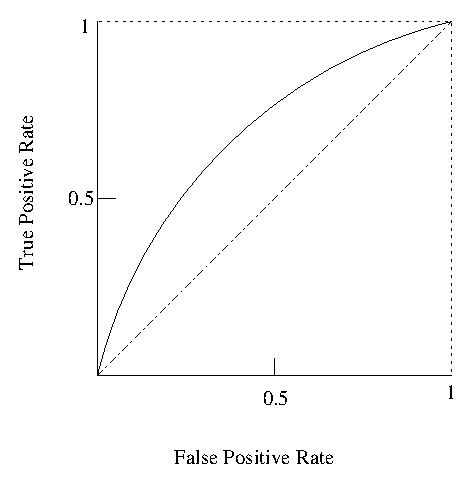
\epsfig{%
    file=./figs/roc.eps,
    %width=.98\columnwidth
    }%
  \caption{ROC Curve}
  \label{fig:roc}%
\end{figure}


These measures have been used to compare the accuracy of the classifiers with and without applying the sampling and FS techniques
explored in this paper.


%%%%%%%%%%%%%%%%%%%%%%%%%%%%%%%%%%%%%%%%%%%%%%%%%%%%%%%%%%%%%%%%%%%%%%%%%%
%%%%%%%%%%%%%%%%%%%%%%%%%%%%%%%%%%%%%%%%%%%%%%%%%%% Experimental Results %
%%%%%%%%%%%%%%%%%%%%%%%%%%%%%%%%%%%%%%%%%%%%%%%%%%%%%%%%%%%%%%%%%%%%%%%%%%

\section{Experimental Results}
\label{sec:experimentalResults}

In this paper, we have applied FS and sampling techniques to the CM1, JM1, KC1, KC2, and PC1 datasets available in the PROMISE
repository~\cite{PROMISERep} in order to generate classification models for finding software defective modules. These datasets were created from projects carried out at NASA and collected under their metrics programme\footnote{\texttt{http://mdp.ivv.nasa.gov/}} and reasons for their selection include: (i) they have been used in
other studies (for example,~\cite{Li+Reformat:2007,MenziesEtAl04,MenziesEtAl07} with a variety of learning methods and techniques for the same purpose, i.e., prediction of defective modules); (ii) all these datasets have a binary class (defective vs. non-defective modules); and (iii) the class is highly unbalanced. Table~\ref{tab:attr} summarises the number of instances, number of non-defective modules, defective modules and percentage of defective modules for each of the previously mentioned datasets.

%CM1 is a NASA spacecraft instrument written in "C"
%JM1 is written in "C" and is a real-time predictive ground system:
%        Uses simulations to generate predictions
%KC1 is a "C++" system implementing storage management for
%       receiving and processing ground data
%KC2 Data from C++ functions. Science data processing; another part
%    of the same project as KC1; different personnel than KC1.  Shared
%    some third-party software libraries with KC1, but no other software
%    overlap.
%PC1 Data from C  functions. flight software for earth orbiting satellite.

%The number of instances, however, varies among the datasets: CM1 %contains 498 instances; JM1, 10885; KC1, 2109; KC2, 522; and PC1 %is composed of 1109 instances.
\begin{table}%[h!]
\begin{center}
\begin{small}
 \caption{No. of Instances per Dataset}
% \emph{Dataset} &  \emph{No. of instances} \\
\begin{tabular}{l|rrrrrr}
\hline
 \emph{Dataset} & \emph{\# instances} & \emph{non-defective} & \emph{defective} & \emph{\% defective} & \emph{Language}\\
\hline \hline
       CM1 &    498 &   449 &    49 &  9.83 & C \\
       JM1 & 10,885 & 8,779 & 2,106 & 19.34 & C \\
       KC1 &  2,109 & 1,783 &   326 & 15.45 & C++ \\
       KC2 &    522 &   415 &   107 & 20.49 & C++ \\
       PC1 &  1,109 & 1,032 &    77 &  6.94 & C \\
\hline
\end{tabular}
\end{small}
 \label{tab:attr}
 \end{center}
\end{table}


All these five datasets also contain the same 22 attributes: 5 different lines of code measure, 3 McCabe metrics~\cite{mccabe76}, 4 base Halstead measures~\cite{halstead77}, 8 derived Halstead measures~\cite{halstead77}, a branch-count, and the class attribute
indicating whether the module has reported defects (Table~\ref{tab:attrDef}). For a comprehensive coverage and explanation of these metrics, we refer to Fenton and Pfleeger~\cite{fenton97}. We have also performed the experiments without the derived attributes but results showed that derived attributes can be more informative than non derived (base) attributes.


\begin{table}%[h!]
\begin{center}
\begin{scriptsize}
\caption{Definition of the Attributes}
\begin{tabular}{l|l|l|l}
\hline
          &   \emph{\#} & \emph{Symbol} &  \emph{Metric} \\
\hline
\hline
    McCabe  &          1 &         loc  &  McCabe's  Lines of code \\
\hline
            &          2 &        v(g)  &  cyclomatic complexity \\
            &          3 &       ev(g)  &  essential complexity \\
            &          4 &       iv(g)  &  design complexity \\
\hline
Halstead Derived  &    5 &           n  &  Total operators + operands \\
                  &    6 &           v  &      volume \\
                  &    7 &           l  &  Program length \\
                  &    8 &           d  &  Difficulty \\
                  &    9 &           i  &  Intelligence \\
                  &   10 &           e  &  Effort \\
                  &   11 &           b  &   Halstead \\
                  &   12 &           t  &  Time estimator \\
                  &   13 &      lOCode  &  Line count \\
                  &   14 &   lOComment  &  Count of lines of comments \\
                  &   15 &     lOBlank  &  Count of blank lines \\
                  &   16 &   lOCodeAndComment  &             \\
\hline
Halstead base  &      17 &     uniq\_Op  &  Unique operators \\
               &      18 &   uniq\_Opnd  &  Unique operands \\
               &      19 &    total\_Op  &  Total operators \\
               &      20 &   total\_Opnd  &  Total operands \\
\hline
     Branch  &        21 &   branchCount  &  No. branches of the flow graph \\
\hline
     Class  &            &     {false, true}  &  Whether the module has reported defects \\
\hline
\end{tabular}
\end{scriptsize}
 \label{tab:attrDef}
 \end{center}
\end{table}


The experiments performed here were conducted using algorithms implemented by the Weka environment~\cite{WF05}, either using the
Explorer or the Experimenter tools. As balancing techniques, the \emph{Resample} and \emph{SpreadSubsample} algorithms were performed to generate the new datasets. With \emph{Resample}, the parameter were set to double the number of instances following a uniform distribution with the class. On the other hand, with \emph{SpreadSubsample}, new datasets were generated removing
instances randomly from the majority class so there is also an approximate equal number of instances for each class but in the
lower end.

Then, FS was performed on the original as well as the new generated datasets using Weka's Experimenter. It is worth noting that these new balanced datasets were generated before the FS techniques. As stated previously, FS can be grouped into filter or wrapper depending on whether the classifier is used to find the feature subset. In this paper, for the filter models, we have applied correlation (CFS)~\cite{Hall99CFSThesis} and consistency (CNS)~\cite{DLM00} evaluators with greedy search (sequential forward - sf) in both cases. For the wrapper-method, the same classifier is used for both feature selection and prediction, in this case, the Na\"ive Bayes (NB).

The results reported in Tables~\ref{tab:NBCorrectAUC} and \ref{tab:NBTNrfmesure} were obtained with ten runs and each run is a
ten-fold cross-validation, i.e., in one run, a feature subset was selected using the 90\% of the instances, then, the accuracy of this subset was estimated over the unseen 10\% of the data. This was performed 10 times, each time proposing a possible different feature subset. In this way, estimated accuracies, selected attribute numbers and time needed were the result of a mean over ten
ten--cross-validation samples.

Also, with a single ten-cross validation run, Table~\ref{tab:noOfTimesAttr} shows the number of times that an attribute has been selected for the CFS-sf (correlation with sequential search - greedy stepwise) algorithm. From software engineering point of view, this it possible to analyse this table in its two dimensions. First, analysing columns in order to find which attributes are important for each dataset and if attributes differ after applying a sampling technique. Second, analyzing rows, it is possible to find which attributes are important across different datasets. For example, it can be observed in Table~\ref{tab:noOfTimesAttr} that for the CM1 dataset, the selected subsets of attributes differ before and after sampling using CFS-fs.
With the original dataset, the main relevant attributes are 1 (McCabe's LOC), 4 (McCabe's Design Complexity -- \texttt{iv(g)}), 9
(Halstead's Intelligence --\texttt{i}), 14 (Halstead's Count of lines of comments) and 17 (Halstead's Unique Operators --
\texttt{uniq\_Op}) with a percentage of correct accuracy of 60, 70, 100, 100 and 60\%. However, with the balanced dataset the most
relevant attributes are 6 (Halstead's volumen --\texttt{v}), 8 (Halstead's Difficulty ), 9 (Halstead's Intelligence --\texttt{i}),
14 (Halstead's Count of lines of comments) y 17 (Halstead's Unique Operators). As it can be observed, they only have three common
attributes and these new attributes have a positive effect in the AUC results and $TN_{rate}$ achieved by the NB classifier (see
Tables~\ref{tab:NBCorrectAUC} and \ref{tab:NBTNrfmesure}).

Analysing rows, the last column of Table~\ref{tab:noOfTimesAttr} shows the total number of times an attribute has been selected.
Therefore, the 3 main attributes are number 9 (Halstead's Intelligence --i), 14 (Halstead's Count of lines of comments) and 15
(Count of blank lines) are able to predict defective modules across all datasets. From the software engineering point of view, it seems strange that lines of comments and blanks are able to indicate which modules will be defective, but project manager could check if this is specific to the domain of the application, organization and if these results can be generalised.

\begin{table}[t]
\caption{No. of Times Attributes has been Selected by the FS
algorithm (CFS)} \label{tab:noOfTimesAttr}
%\vskip 0.15in
\begin{center}
\begin{scriptsize}
\begin{tabular}{r|rrr|rrr|rrr|rrr|rrr|r}
\hline
\multicolumn{1}{c}{}& \multicolumn{3}{c}{CM1} & \multicolumn{3}{c}{JM1} & \multicolumn{3}{c}{KC1} & \multicolumn{3}{c}{KC2} & \multicolumn{3}{c}{PC1} \\
\hline
   \emph{\#}& \emph{Ori} & \emph{Rs} & \emph{Sp} & \emph{Or} & \emph{Rs} & \emph{Sp} &  \emph{Ori} &  \emph{Rs} &  \emph{Sp} &  \emph{Ori} &   \emph{Rs} &  \emph{Sp} &  \emph{Ori} &  \emph{Rs} &  \emph{Sp} & \emph{Sum}\\
\hline \hline
  1 &   6 &    0 &  0 &  10 &   10 &  10 &   1 &  10 &  10 &   4 &   7 &  10 &   1 &   0 &   0  & 97\\
  2 &   0 &    0 &  0 &   4 &    7 &   3 &   4 &   0 &   1 &   0 &   0 &   0 &   2 &   0 &   0 & 21\\
  3 &   0 &    0 &  0 &  10 &   10 &   5 &   2 &  10 &   0 &  10 &  10 &  10 &   0 &   0 &   0 & 67\\
  4 &   7 &    0 &  4 &  10 &   10 &  10 &   1 &   0 &   0 &   0 &   0 &   0 &   0 &   0 &   0 & 42\\
  5 &   0 &    0 &  0 &   0 &    0 &   0 &   1 &   0 &   6 &   2 &   1 &   2 &   0 &   0 &   0 & 12\\
  6 &   0 &   10 &  2 &   0 &    9 &   0 &   0 &   2 &   4 &   0 &   4 &   0 &   0 &  10 &   0 & 41\\
  7 &   0 &    0 &  0 &   0 &    0 &   4 &   0 &   1 &   0 &   0 &   0 &   0 &   0 &   0 &   0 &  5\\
  8 &   1 &    9 &  0 &   0 &    0 &   0 &   8 &   9 &   2 &   2 &   9 &   0 &   0 &   0 &   0 & 40\\
  9 &  10 &   10 &  6 &  10 &   10 &  10 &  10 &  10 &  10 &  10 &   9 &  10 &   5 &  10 &  10 & 140\\
  10 &   0 &    0 &  2 &   0 &    1 &   0 &   4 &   2 &   4 &   0 &   0 &   1 &   0 &   0 &   2 & 16\\
  11 &   1 &    0 &  6 &   0 &    0 &   0 &   0 &   0 &   0 &   0 &   6 &   6 &   0 &   0 &   0 & 19\\
  12 &   0 &    0 &  0 &   0 &    0 &   0 &   2 &   5 &   0 &   0 &   0 &   0 &   0 &   3 &   0 & 10\\
  13 &   1 &    0 &  0 &   0 &    0 &   0 &   6 &  10 &   4 &   1 &   3 &   0 &   1 &   0 &   0 & 26\\
  14 &  10 &   10 &  9 &  10 &   10 &  10 &   9 &   2 &   0 &   2 &  10 &   7 &   9 &   0 &   0 & 98 \\
  15 &   4 &    1 &  8 &  10 &   10 &   9 &  10 &  10 &   4 &   2 &   1 &   9 &  10 &   0 &   0 & 88\\
  16 &   0 &    0 &  0 &  10 &   10 &  10 &   0 &   0 &   0 &   4 &   0 &   2 &  10 &   0 &  10 & 56\\
  17 &   6 &    5 &  0 &   0 &    0 &   0 &   1 &   0 &   1 &   8 &   1 &   1 &   0 &   0 &  10 & 33\\
  18 &   4 &    0 &  0 &   0 &    0 &   1 &   7 &   0 &   0 &  10 &   9 &  10 &   4 &   0 &   1 & 46\\
  19 &   0 &    0 &  1 &   0 &    0 &   1 &   0 &   0 &   6 &   0 &   0 &   1 &   1 &   0 &   0 & 10\\
  20 &   0 &    0 &  0 &   0 &    0 &   1 &   4 &   4 &   3 &   0 &   0 &   3 &   0 &   0 &   0 & 15\\
  21 &   0 &    0 &  0 &   6 &    3 &   7 &   8 &   0 &   6 &   0 &   0 &   0 &   0 &   0 &   0 & 30\\
\hline
\multicolumn{17}{l}{\scriptsize \emph{Ori}, Original; \emph{Rs}, Resample; \emph{Sp}, SpreadSubsample}\\
\end{tabular}
\end{scriptsize}
\end{center}
%\vskip -0.1in
\end{table}



\begin{table}[t]
\caption{NB Percentage of Correct and AUC} \label{tab:NBCorrectAUC}
%\vskip 0.15in
\begin{center}
\begin{small}
\begin{tabular}{r|rrrr|rrrr}
\hline
\multicolumn{ 1}{c}{} & \multicolumn{ 4}{c}{\emph{\% Correct}} &  \multicolumn{ 4}{c}{\emph{AUC}} \\
\hline
 & \emph{Ori} & \emph{CFS} & \emph{CNS} & \emph{WP} & \emph{Ori} & \emph{CFS} & \emph{CNS} & \emph{WP} \\
\hline \hline
     CM1 & 84.84 &  87.15 &  89.70 &  90.02 &  0.74 &  0.74 &  0.52 & 0.52  \\
 CM1$_A$ & 61.23 &  62.32 &  62.16 &  71.43 &  0.76 &  0.76 &  0.75 & 0.78  \\
 CM1$_B$ & 63.03 &  63.31 &  62.61 &  59.70 &  0.67 &  0.65 &  0.65 & 0.67 \\
     JM1 & 80.42 &  80.37 &  80.34 &  80.67 &  0.69 &  0.67 &  0.69 & 0.63  \\
 JM1$_A$ & 58.01 &  59.20 &  58.50 &  61.68 &  0.69 &  0.67 &  0.69 & 0.69  \\
 JM1$_B$ & 57.86 &  59.42 &  58.34 &  61.15 &  0.69 &  0.67 &  0.69 & 0.68 \\
     KC1 & 82.46 &  82.73 &  82.30 &  85.38 &  0.79 &  0.79 &  0.79 & 0.79 \\
 KC1$_A$ & 64.46 &  64.30 &  64.43 &  71.16 &  0.79 &  0.80 &  0.80 & 0.78  \\
 KC1$_B$ & 62.30 &  62.30 &  62.87 &  68.73 &  0.77 &  0.77 &  0.77 & 0.76 \\
     KC2 & 83.62 &  83.60 &  83.97 &  83.24 &  0.84 &  0.84 &  0.84 & 0.83 \\
 KC2$_A$ & 66.04 &  68.13 &  66.37 &  77.99 &  0.85 &  0.84 &  0.84 & 0.84  \\
 KC2$_B$ & 67.20 &  68.55 &  68.65 &  74.73 &  0.83 &  0.83 &  0.83 & 0.83 \\
     PC1 & 89.00 &  90.05 &  88.74 &  92.89 &  0.71 &  0.75 &  0.73 & 0.52  \\
 PC1$_A$ & 60.42 &  58.24 &  59.23 &  63.11 &  0.71 &  0.69 &  0.66 & 0.74  \\
 PC1$_B$ & 64.27 &  67.17 &  67.19 &  68.55 &  0.72 &  0.80 &  0.79 & 0.78  \\
\hline
%\footnotesize
\multicolumn{9}{l}{\scriptsize $_{A}$, Resample; $_{B}$, SpreadSub.}\\
\multicolumn{9}{l}{\scriptsize \emph{Ori}, Original; \emph{CFS}, Correlation; \emph{CNS}, Consistency; \emph{WP}, Wrapper.}\\
\end{tabular}
\end{small}
\end{center}
%\vskip -0.1in
\end{table}



\begin{table}[t]
\caption{True Negative Rate, $TN_{rate}$ (Defective Modules) and
$f-measure$ Values} \label{tab:NBTNrfmesure}
%\vskip 0.15in
\begin{center}
\begin{small}\begin{tabular}{r|rrrr|rrrr}
\hline
 \multicolumn{ 1}{c}{} & \multicolumn{4}{c}{\emph{True Negative Rate}} & \multicolumn{4}{c}{\emph{f-measure}} \\
\hline
 & \emph{Ori} & \emph{CFS} & \emph{CNS} & \emph{WP} & \emph{Ori} & \emph{CFS} & \emph{CNS} & \emph{WP} \\
\hline \hline
     CM1 &  0.30 &  0.28 &  0.01 &   0.00  &    0.91 &   0.93 &  0.95 &  0.95  \\
 CM1$_A$ &  0.35 &  0.37 &  0.37 &   0.66  &    0.69 &   0.69 &  0.69 &  0.72  \\
 CM1$_B$ &  0.35 &  0.37 &  0.36 &   0.37  &    0.71 &   0.71 &  0.70 &  0.66 \\
     JM1 &  0.20 &  0.22 &  0.21 &   0.14  &    0.89 &   0.89 &  0.89 &  0.89  \\
 JM1$_A$ &  0.21 &  0.24 &  0.23 &   0.33  &    0.69 &   0.70 &  0.69 &  0.70  \\
 JM1$_B$ &  0.21 &  0.25 &  0.22 &   0.30  &    0.69 &   0.70 &  0.69 &  0.70  \\
     KC1 &  0.37 &  0.35 &  0.38 &   0.22  &    0.90 &   0.90 &  0.90 &  0.92  \\
 KC1$_A$ &  0.38 &  0.39 &  0.39 &   0.68  &    0.72 &   0.71 &  0.72 &  0.72 \\
 KC1$_B$ &  0.37 &  0.37 &  0.39 &   0.69  &    0.70 &   0.70 &  0.70 &  0.69 \\
     KC2 &  0.41 &  0.44 &  0.45 &   0.40  &    0.90 &   0.90 &  0.90 &  0.90 \\
 KC2$_A$ &  0.40 &  0.45 &  0.41 &   0.73  &    0.73 &   0.74 &  0.73 &  0.78  \\
 KC2$_B$ &  0.39 &  0.42 &  0.43 &   0.68  &    0.75 &   0.75 &  0.75 &  0.76 \\
     PC1 &  0.30 &  0.31 &  0.30 &   0.01  &    0.94 &   0.95 &  0.94 &  0.96  \\
 PC1$_A$ &  0.31 &  0.27 &  0.29 &   0.35  &    0.69 &   0.68 &  0.69 &  0.71  \\
 PC1$_B$ &  0.34 &  0.41 &  0.42 &   0.46  &    0.73 &   0.74 &  0.74 &  0.75 \\
\hline
%\footnotesize
\multicolumn{9}{l}{\scriptsize $_{A}$, Resample; $_{B}$, SpreadSub.}\\
\multicolumn{9}{l}{\scriptsize \emph{Ori}, Original; \emph{CFS}, Correlation; \emph{CNS}, Consistency; \emph{WP}, Wrapper.}\\
\end{tabular}
\end{small}
\end{center}
%\vskip -0.1in
\end{table}




%
%\begin{table}[t]
%\caption{NB. True Negative Rate, $TN_{rate}$ (Defective Modules)}
%\label{tab:mesures}
%%\vskip 0.15in
%\begin{center}
%\begin{tiny}\begin{tabular}{r|rrrr|rrrr|rrrr|rrrr}
%\hline
% \multicolumn{1}{c}{} & \multicolumn{4}{c}{\emph{True Negative Rate}} & \multicolumn{4}{c}{\emph{f-measure}} & \multicolumn{4}{c}{\emph{True Negative Rate}}& \multicolumn{4}{c}{\emph{True Negative Rate}}\\
%\hline
% & \emph{Ori} & \emph{CFS} & \emph{CNS} & \emph{WP} & \emph{Ori} & \emph{CFS} & \emph{CNS} & \emph{WP} & \emph{Ori} & \emph{CFS} & \emph{CNS} & \emph{WP} & \emph{Ori} & \emph{CFS} & \emph{CNS} & \emph{WP}\\
%\hline \hline
%     CM1  &      84.84 &      87.15 &       89.7 &      90.02 &       0.74 &       0.74 &       0.52 &       0.52 &        0.3 &       0.28 &       0.01 &          0 &       0.91 &       0.93 &       0.95 &       0.95 \\
% CM1$_A$  &      61.23 &      62.32 &      62.16 &      71.43 &       0.76 &       0.76 &       0.75 &       0.78 &       0.35 &       0.37 &       0.37 &       0.66 &       0.69 &       0.69 &       0.69 &       0.72 \\
% CM1$_B$  &      63.03 &      63.31 &      62.61 &       59.7 &       0.67 &       0.65 &       0.65 &       0.67 &       0.35 &       0.37 &       0.36 &       0.37 &       0.71 &       0.71 &        0.7 &       0.66 \\
%     JM1  &      80.42 &      80.37 &      80.34 &      80.67 &       0.69 &       0.67 &       0.69 &       0.63 &        0.2 &       0.22 &       0.21 &       0.14 &       0.89 &       0.89 &       0.89 &       0.89 \\
% JM1$_A$  &      58.01 &       59.2 &       58.5 &      61.68 &       0.69 &       0.67 &       0.69 &       0.69 &       0.21 &       0.24 &       0.23 &       0.33 &       0.69 &        0.7 &       0.69 &        0.7 \\
% JM1$_B$  &      57.86 &      59.42 &      58.34 &      61.15 &       0.69 &       0.67 &       0.69 &       0.68 &       0.21 &       0.25 &       0.22 &        0.3 &       0.69 &        0.7 &       0.69 &        0.7 \\
%     KC1  &      82.46 &      82.73 &       82.3 &      85.38 &       0.79 &       0.79 &       0.79 &       0.79 &       0.37 &       0.35 &       0.38 &       0.22 &        0.9 &        0.9 &        0.9 &       0.92 \\
% KC1$_A$  &      64.46 &       64.3 &      64.43 &      71.16 &       0.79 &        0.8 &        0.8 &       0.78 &       0.38 &       0.39 &       0.39 &       0.68 &       0.72 &       0.71 &       0.72 &       0.72 \\
% KC1$_B$  &       62.3 &       62.3 &      62.87 &      68.73 &       0.77 &       0.77 &       0.77 &       0.76 &       0.37 &       0.37 &       0.39 &       0.69 &        0.7 &        0.7 &        0.7 &       0.69 \\
%     KC2  &      83.62 &       83.6 &      83.97 &      83.24 &       0.84 &       0.84 &       0.84 &       0.83 &       0.41 &       0.44 &       0.45 &        0.4 &        0.9 &        0.9 &        0.9 &        0.9 \\
% KC2$_A$  &      66.04 &      68.13 &      66.37 &      77.99 &       0.85 &       0.84 &       0.84 &       0.84 &        0.4 &       0.45 &       0.41 &       0.73 &       0.73 &       0.74 &       0.73 &       0.78 \\
% KC2$_B$  &       67.2 &      68.55 &      68.65 &      74.73 &       0.83 &       0.83 &       0.83 &       0.83 &       0.39 &       0.42 &       0.43 &       0.68 &       0.75 &       0.75 &       0.75 &       0.76 \\
%     PC1  &         89 &      90.05 &      88.74 &      92.89 &       0.71 &       0.75 &       0.73 &       0.52 &        0.3 &       0.31 &        0.3 &       0.01 &       0.94 &       0.95 &       0.94 &       0.96 \\
% PC1$_A$  &      60.42 &      58.24 &      59.23 &      63.11 &       0.71 &       0.69 &       0.66 &       0.74 &       0.31 &       0.27 &       0.29 &       0.35 &       0.69 &       0.68 &       0.69 &       0.71 \\
% PC1$_B$  &      64.27 &      67.17 &      67.19 &      68.55 &       0.72 &        0.8 &       0.79 &       0.78 &       0.34 &       0.41 &       0.42 &       0.46 &       0.73 &       0.74 &       0.74 &       0.75 \\
%\hline
%%\footnotesize
%\multicolumn{17}{l}{\tiny $_{A}$, Resample; $_{B}$, SpreadSub.}\\
%\multicolumn{17}{l}{\tiny Ori, Original; CFS, Correlation; CNS, Consistency; WP, Wrapper.}\\
%\end{tabular}
%\end{tiny}
%\end{center}
%%\vskip -0.1in
%\end{table}


Also, a multifactorial ANOVA was performed to test the significance of the FS methods used and the effect of sampling techniques. With $\alpha$-level of 0.5, both FS, resampling and their interaction have a significant effect in the variables AUC and true negatives rate ($TN_{rate}$). The effect of the \emph{wrapper} model is especially significant for both variables, as showed in
Figure~\ref{fig:AnovaMeanFS} for the percentage of true negatives (finding defective modules).


\begin{figure}%[tb]
  \centering
  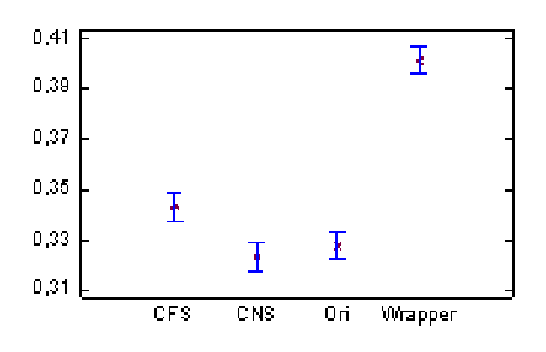
\epsfig{%
    file=./figs/analysis1.eps,
    %width=.85\columnwidth
    }%
  \caption{Mean $TN_{rate}$ vs. Feature Selection}
  \label{fig:AnovaMeanFS}%
\end{figure}

Sampling techniques have also an important effect in the percentage of true negatives in general. The most significant effect in that parameter is the interaction of the \emph{Wrapper} method with \emph{Resample} technique, accounting for an statistically
significant difference in the mean from the base case higher than 24\% (Figure~\ref{fig:AnovaMeanSampling}).

\begin{figure}%[tb]
  \centering
  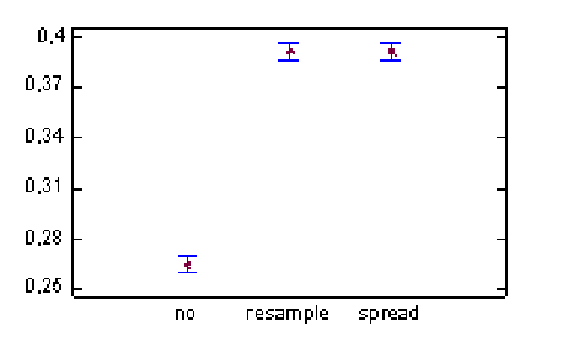
\epsfig{%
    file=./figs/analysis2.eps,
    %width=.98\columnwidth
    }%
  \caption{Mean $TN_{rate}$ vs. Sampling techniques}
  \label{fig:AnovaMeanSampling}%
\end{figure}

%\begin{figure}[htbp]
%\centerline{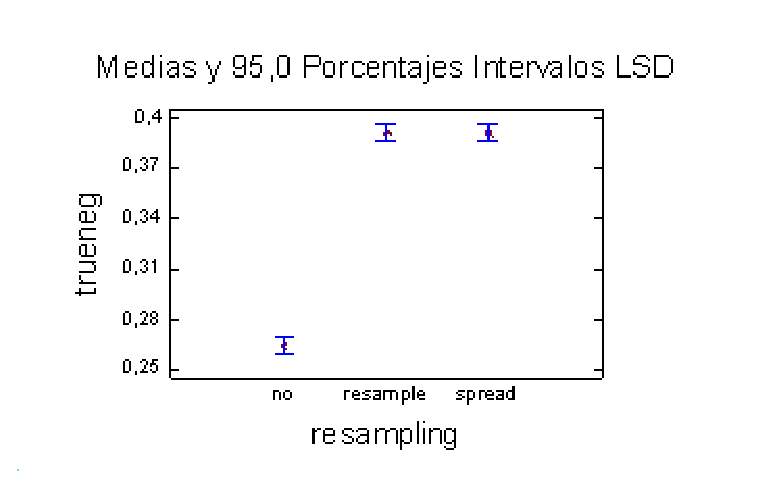
\includegraphics[width=4.89in,height=3.05in]{figs/analisis2.eps}}
%\label{fig2}
%\end{figure}



%
%\begin{figure}[h]
%  \hfill
%  \begin{minipage}[t]{.45\textwidth}
%    \begin{center}
%      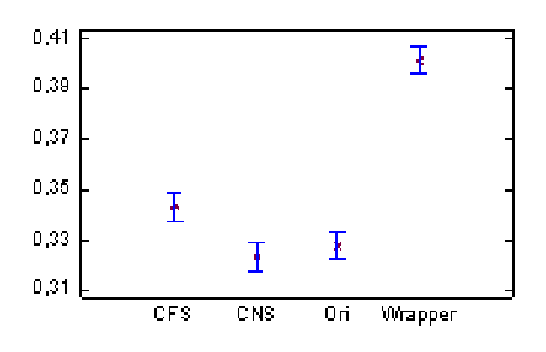
\epsfig{file=figs/analysis1.eps, scale=0.8}
%      \caption{figure 1}
%      \label{fig-tc}
%    \end{center}
%  \end{minipage}
%  \hfill
%  \begin{minipage}[t]{.45\textwidth}
%    \begin{center}
%      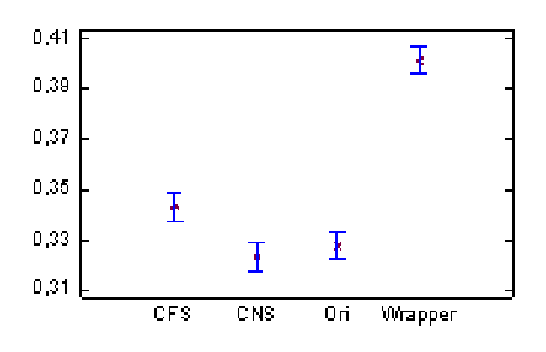
\epsfig{file=figs/analysis1.eps, scale=0.8}
%      \caption{figure 2}
%      \label{fig-tc}
%    \end{center}
%  \end{minipage}
%  \hfill
%\end{figure}

%
%\begin{figure}[htbp]
%  \begin{center}
%    \mbox{
%      \subfigure[a]{\scalebox{0.75}{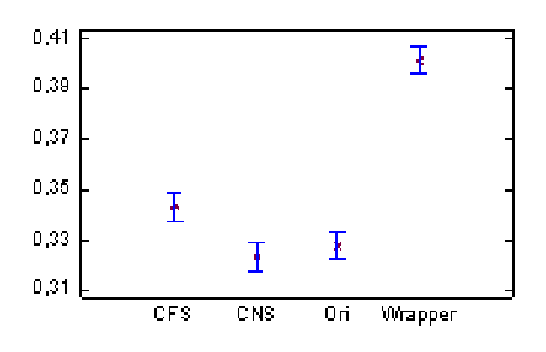
\epsfig{file=figs/analysis1.eps}}} \quad
%      \subfigure[b]{\scalebox{0.75}{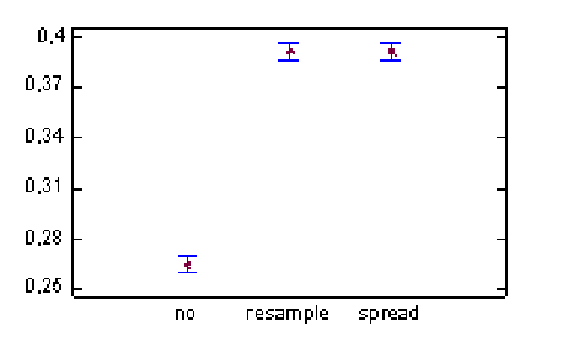
\epsfig{file=figs/analysis2.eps}}}
%      }
%    \caption{I like these!}
%    \label{fig:fig:anova}
%  \end{center}
%\end{figure}


Although the overall accuracy does not seem to generally improve, ANOVA analysis shows that sampling techniques improve the prediction of defective modules, i.e., the ones we are interested in finding. This can also be corroborated visually observing
Tables~\ref{tab:NBCorrectAUC} and \ref{tab:NBTNrfmesure}, which show different measurements of the goodness of classification results. In relation to feature selection, a smaller number of attributes is capable of maintaining the prediction capability with a lower number of attributes than the original datasets and also allow us to characterise the datasets.


We also need to consider the threads to validity \cite{fenton97,WohlinEtAl2000experimentation} of this study:

\begin{itemize}
  \item \emph{Construct validity}. It is the degree to which the variables used in the study accurately measure the concepts they purport to measure. It may happens that the metrics used do not adequately capture the purpose for which they were design. There is some controversy whether the metrics of the datasets used in this work are useful indicators. For example, Fenton and Pfleeger reported that Cyclomatic complexity is a and Lines of Code are highly correlated~\cite{fenton97}. Also, as we have seen, some of the metrics selected by the feature selection algorithm seem to be counterintuitive as predictors of defective
modules (e.g., Lines of comments or blanks, etc.).

\item \emph{Internal validity}. It is the degree to which conclusions can be drawn about the causal effect of the independent variable on the dependent variables. This thread was minimized using a variety of filters, and measurement techniques. It is worth noting that NB is quite robust to independency and normality distribution of the variables, as a result there was no transformation of variables before the learning algorithm.
%It is worth noting that we did not transform the input variables as
%in other studies (for example, Menzies et al~\cite{MenziesEtAl07}
%use log transformations with the NB classifier), although the NB
%classifier assumes independency and normality of the independent
%variables, it is quite robust when it is not the case.
In relation to balancing techniques used in this work, we also need to consider that \emph{Resampling} increases the number of intances through replication, perhaps increasing the effect of overfitting.

\item \emph{External validity}. It is the degree to which the results of the research can be generalised to the population under study and other research settings. It is believed that results can be generalised~\cite{MenziesEtAl07,BasiliEtAl:2002}. They are, however, specific to a very concrete domain. Further studies are needed to corroborate all these issues.

\end{itemize}


%%%%%%%%%%%%%%%%%%%%%%%%%%%%%%%%%%%%%%%%%%%%%%%%%%%%%%%%%%%%%%%%%%%%%
%%%%%%%%%%%%%%%%%%%%%%%%%%%%%%%%%%%%%%%%%%%%%%%%%%%%%% Related Work %
%%%%%%%%%%%%%%%%%%%%%%%%%%%%%%%%%%%%%%%%%%%%%%%%%%%%%%%%%%%%%%%%%%%%%

\section{Related Work}
\label{sec:relatedWork}

Until now, few authors have investigated the application of FS to software engineering datasets areas such as cost estimation or
quality. Among these works, Chen et al~\cite{ChenEtAl:05} have analyzed the application of FS using wrappers to the problem of cost estimation. They also concluded that the reduced dataset could improve the estimation. Kirsopp and Shepperd~\cite{kirsoppShepperd:02} have also analyzed the application of FS to cost estimation reaching with similar conclusions.

Sampling techniques are known to improve the accuracy results of balance datasets. For example, Seiffert et al~\cite{SeiffertEtAl07} reported on the effect of noise with different sampling techniques have with different learners. The sampling techniques used include Random undersampling (RUS), random oversampling (ROS), one-sided selection (OSS), cluster-based oversampling (CBOS), Wilson's editing (WE), SMOTE (SM), and borderline-SMOTE (BSM). Authors conclude there is that some sampling techniques are more robust to noise (RUS, WE and BSM) than others (ROS and SM) and the level of imbalance also affects the sampling technique. Authors used a single publicly available dataset where noise was artificially injected at different levels. This work has been extended by Van Hulse, Khoshgoftaar and Napolitano~\cite{VanHulse+EtAl:2007} to further analyse the effect of unbalance dataset with a much larger number of learners and databases mainly form the UCI repository~\cite{Asuncion+Newman:2007}.

In relation to balancing techniques in software engineering, Yasutaka et al.~\cite{YasutakaEtAl:07} analysed the application of
four sampling techniques (ROS, SMOTE, RUS, and ONESS) for classifying defective modules with also four different types of
models (Linear Discriminant Analysis -- LDA, Logistic Regression -- LR Analysis, Neural Networks -- NN and Classification Trees -- CT) in a single Management Information System software. Authors concluded that sampling does not improve the performance of NN and
CT models and the improvements with the other two, LDA and LR, depend on the level of sampling. These conclusions were based on a
single measure, the $f-measure$ and evaluation procedure was preformed without cross-validation, just dividing the dataset into
training and testing. Li and Reformat~\cite{Li+Reformat:2007} have also approached the problem of unbalanced datasets combining
learners and fuzzy logic to generate models that are more robust to this problem.


%%%%%%%%%%%%%%%%%%%%%%%%%%%%%%%%%%%%%%%%%%%%%%%%%%%%%%%%%%%%%%%%%%%%%%%%%%
%%%%%%%%%%%%%%%%%%%%%%%%%%%%%%%%%%%%%%%%%%%%%%%%%%%%%%%%% Conclusions %%%%
%%%%%%%%%%%%%%%%%%%%%%%%%%%%%%%%%%%%%%%%%%%%%%%%%%%%%%%%%%%%%%%%%%%%%%%%%%

\section{Conclusions and Future Work}
\label{sec:conclusions}


In this paper, different Feature Selection (FS) and balancing techniques were applied to different datasets from the PROMISE
repository as a preprocesing techniques in order to generate Na\"ive Bayes classifiers in order to predict defective modules. The results of the analysis performed here provides evidence on the impact of balancing techniques methods on detecting defective modules combined or not with FS, which points to the methodological adequacy of using balancing techniques to alleviate the effect of unbalanced datasets. In relation to FS, the reduced datasets maintain the prediction capability with a lower number of attributes than the original datasets.

Future work will be performed using other kinds of metrics and domains. We will also include further techniques and different
datasets as a way of generalising conclusions about how to preprocess software engineering datasets.  We will also intend to extend this work to further datasets with different metrics (e.g., object-oriented metrics), problems with more than two classes and numeric prediction. We indent to use other datasets and specifically some with object oriented metrics from the Promise
repository. Finally, FS and balancing techniques are only two of the techniques that can be used for preprocessing datasets. There are other techniques to remove outliers, noise, etc. that can be used in combination with these techniques.

%different software engineering problems such as estimation. In
%addition, a possible problem with the analyzed datasets is that some
%of the datasets are imbalanced, i.e., many more modules were
%classified as non-defective than defective. Current research works
%on how to balance dataset can be applied before the techniques
%described here.

%%%%%%%%%%%%%%%%%%%%%%%%%%%%%%%%%%%%%%%%%%%%%%%%%%%%%%%%%%%%%%%%%%%%%%%%%%
%%%%%%%%%%%%%%%%%%%%%%%%%%%%%%%%%%%%%%%%%%%%%%%%%%%%% Acknoledgements %%%%
%%%%%%%%%%%%%%%%%%%%%%%%%%%%%%%%%%%%%%%%%%%%%%%%%%%%%%%%%%%%%%%%%%%%%%%%%%

%\section*{Acknowledgements}
%
%%We would like to thank the Spanish Ministry of Science and
%%Technology for supporting this research (Project CICYT
%%TIN2004-06689-C03).


%-------------------------------------------------------------------------
%\nocite{ex1,ex2}
\bibliographystyle{elsart-num-sort}
\bibliography{./references/references}


\end{document}
